\capitulo{4}{Técnicas y herramientas}

%Esta parte de la memoria tiene como objetivo presentar las técnicas metodológicas y las herramientas de desarrollo que se han utilizado para llevar a cabo el proyecto. Si se han estudiado diferentes alternativas de metodologías, herramientas, bibliotecas se puede hacer un resumen de los aspectos más destacados de cada alternativa, incluyendo comparativas entre las distintas opciones y una justificación de las elecciones realizadas. 
%No se pretende que este apartado se convierta en un capítulo de un libro dedicado a cada una de las alternativas, sino comentar los aspectos más destacados de cada opción, con un repaso somero a los fundamentos esenciales y referencias bibliográficas para que el lector pueda ampliar su conocimiento sobre el tema.

\section{Java}

Java es un lenguaje de programación desarrollado por James Gosling de Sun Microsystems y publicado en 1995.

Es un lenguaje de programación orientado a objetos, de propósito general y orientado a objetos que fue diseñado con el objetivo de tener la menor cantidad de dependencias de implementación posibles. Un programa java es un programa multiplataforma que solo necesita ser compilado una vez para ser ejecutado en diferentes máquinas. Esto se consigue ya que el programa se ejecuta sobre una máquina virtual java (JVM), elemento que debe estar disponible en el sistema sobre el que se va a ejecutar el programa.

Java cuenta con una gran cantidad de documentación en línea así como una gran variedad de librerías de código abierto creadas por la comunidad que extienden el uso de Java a muchas aplicaciones diferentes, mejorando la funcionalidad original de Java. En este proyecto por ejemplo nos ha servido para realizar la parte de Web Scraping y de la Web Semántica.

Url de la herramienta:

\url{<https://www.java.com/es/download/faq/whatis_java.xml>}

\section{Python}

Python es un lenguaje de programación  interpretado, tipado dinámicamente y multiplataforma. Soporta porgramación orientada a objetos, programación imperativa y en menor medida, programación funcional. Su filosofía hace hincapié en una sintaxis que favorezca un código legible \cite{wiki:python}.

Url de la herramienta: \url{<https://www.python.org/>}

\section{Eclipse}

Eclipse es un entorno de desarrollo integrado (IDE, Integrated Development Environment) disponible para varios lenguajes de programación aunque el de uso más extendido sea el de Java. 

En este proyecto se ha trabajado con el IDE de Java denominado Java EE (Eclipse IDE for Java EE Developers) en su versión "Neon.3".

Url de la herramienta: \url{<https://www.eclipse.org/ide/>}

\section{Apache Maven}

Apache Maven es una herramienta para manejar e interpretar nuestros proyectos software mediante un archivo de configuración XML. Maven se basa en el concepto de \textit{project object model (POM)} para describir como y en que orden se van a construir los elementos de un proyecto y para manejar las dependencias de ese proyecto.

Apache Maven permite manejar estás dependencias por Internet descargando y actualizado los diferentes repositorios \cite{wiki:maven}.

Url de la herramienta: \url{<https://maven.apache.org/>}

\section{Android}

Android es un sistema operativo basado en Linux. Fue diseñado con el objetivo de operar en dispositivos móviles con patalla táctil, empezando por los teléfonos inteligentes y tabletas y después extendiéndose a nuevos dispositivos como relojes inteligentes, televisores y automóviles. Fue desarrollado por Android Inc., empresa respaldada económicamente por Google que en 2005 la compró. Android fue se lanzo en 2007 junto a la fundación Open Handset Alliance, que es un consorcio de compañias hardware, software y de telecomunicaciones \cite{wiki:android}.

Los principales componentes del sistema operativo Android son los siguientes:

\begin{itemize}
	\item{Aplicaciones}: Todas están escritas en el lenguaje de programación Java.
	\item{Marco de trabajo de aplicaciones}: Todos los desarrolladores tienen acceso al mismo entorno de trabajo donde cualquier aplicación puede publicar sus capacidades y luego cualquier otra aplicación puede hacer uso de estas capacidades. Este mecanismo a su vez permite que los componentes sean reemplazados por el usuario.
	\item{Bibliotecas}:Android dispone de una serie de bibiliotecas del sistema escritas en C/C++ cuyas características se ponen a disposición de los desarrolladores a través del marco de trabajo.
	\item{\textit{Runtime} de Android}: Android proporciona un set de librerías que proporcional la funcionalidad base de Java. Cada aplicación se ejecuta en una máquina virtual ART.
	\item{Núcleo Linux}: Android depende de Linux para los servicios base del sistema.
\end{itemize}


Url de la herramienta: \url{<https://developer.android.com/index.html?hl=es-419>}

\section{Android Studio}

Android Studio es el entorno de desarrollo integrado (IDE) oficial de Android. Tiene el objetivo de facilitar el desarrollo en Android proporcionando herramientas personalizadas a los usuarios así como herramientas completas de edición, depuración, pruebas y perfilamiento de código.

Url de la herramienta: \url{<https://developer.android.com/studio/index.html?hl=es-419>}

\section{JavaScript}

JavaScript es un lenguaje de programación orientado a objetos, basado en prototipos, débilmente tipado y dinámico. Puede ser aplicado sobre un documentos HTML con el fin de crear interactividad dinámica con las páginas Web.

JavaScript se desarrollo inicialmente con una sintaxis parecida a C y adopta nombres y convenciones del lenguaje de programación Java \cite{wiki:javascript}.

Url de la herramienta: \url{<https://www.javascript.com/>}

\section{SLF4J}

SLF4J (The Simple Logging Facade for Java) proporciona una API de registro a Java mediante un patrón de fachada que se aplica a varios marcos de registro (\textit{logging frameworks}) que permite al usuario mostrar el marco de registro deseado en el momento de desplieque de la aplicación.

SLF4J nos permite filtrar los mensajes de log para visualizar de una forma más oportuna la información que nos muestra Java.

Url de la herramienta: \url{<https://www.slf4j.org/>}

\section{RDF}

El Resource Description Framework (RDF) es una definición de tipo de documento de XML, es decir, una series de metadatos que usan XML para poder relacionar contenidos entre las diferentes páginas web.

Los objetos de información o recursos se describen a través de un conjunto de propiedades denominadas "descripción RDF" (<rdf:description>). Estas propiedades se pueden entender como atributos de los recursos correspondiéndose a los pares atributo-valor tradicionales.

En el modelo de datos de RDF podemos distinguir tres tipos de objetos:

\begin{itemize}
	\item{Recursos}: Cualquier recurso Web identificado unívocamente por un URI.
	\item{Propiedades}: Son características o atributos usadas para describir los recursos. En ellas se definen los valores permitidos y sobre que recursos se pueden aplicar.
	\item{Descripciones}: Son una triada formada por un recurso, un nombre de propiedad y un valor para esa propiedad. (Sujeto, predicado y objeto).
Ver siguiente figura \ref{figDescripcionRDF}

\begin{figure}[h]
    \begin{center}%
        \begin{center}%
          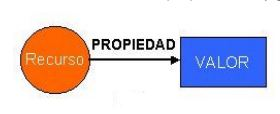
\includegraphics[width=1\textwidth]{DescripcionRDF}%
          \caption{Descripciones RDF.}%
          \label{figDescripcionRDF}%
        \end{center}%
  	\end{center}%
\end{figure}%

\end{itemize}

\newpage
RDF usa la sintaxis básica de XML1.0. Ejemplo: 

"<xmlns:rdf="http://www.w3.org/TR/REC-rdf-syntax">"

El modelo de datos y la sintaxis no son necesarios para definir la relción entre los diferentes recursos y predicados, por ello hace falta un esquema.
Un esquema son una serie de informaciones relativas a la clase a la que pertenecen los recursos para establecer relaciones jerárquicas entre ellos.

\section{Apache Jena}

Apache Jena es un entorno de desarrollo de código abierto para Java cuyo objetivo es el de permitir construir aplicaciones que hagan uso de la Web semántica y del \textit{Linked Data}\footnote{Método por el cuál se publican datos estructurados para que puedan ser interconectados con facilidad.}. 

El framework hace uso de diferentes APIs para extraer y escribir información en grafos RDF\footnote{Modelo de datos para los metadatos basado en triadas de información} \cite{wiki:jena}.

La arquitectura de Apache Jena contempla las siguientes características:

\begin{itemize}
	\item{Arquitectura para manejar (leer, procesar, escribir) las ontologías RDF y OWL.}
	\item{Motor para razonar sobre estas ontologías RDF y OWL.}
	\item{API para almacenar las tripletas RDF en ficheros o en memoria.}
	\item{Motor de queries para realizar consultas bajo la especificación SPARQL \cite{jena}.}
\end{itemize}

En la siguiente figura se muestra un esquema de la arquitectura de Apache Jena.



\begin{figure}[tph]
    \begin{center}%
          \begin{center}%
            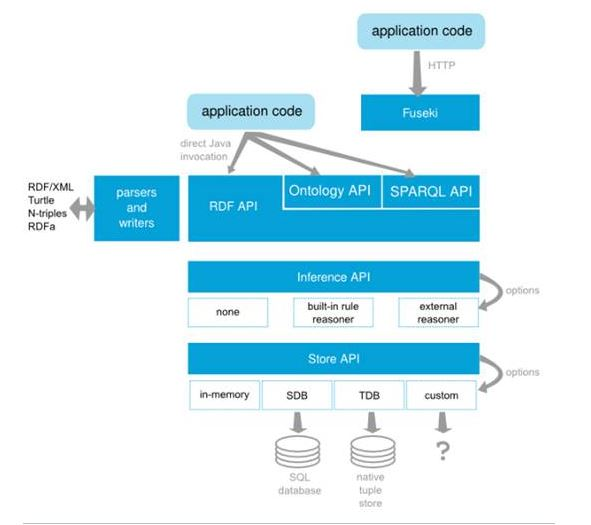
\includegraphics[width=0.8\textwidth]{ApacheJena}%
            \caption{Arquitectura de Apache Jena}%
            \label{figJena}%
          \end{center}%
    \end{center}%
  \end{figure}%

Url de la herramienta: \url{<https://jena.apache.org/>}

\newpage
\section{JSON}

JSON (acrónimo de JavaScrip Object Notation) es un formato de texto ligero para el intercambio de datos. Es un subconjunto de la notación de JavaScript pero debido a la extensión de su uso como alternativa a XML se considera como un formato de lenguaje independiente.

La principal ventaja que ofrece JSON es la fácilidad para crear analizadores sintácticos (\textit{parsers}) \cite{wiki:JSON}.

Url de la herramienta: \url{<https://www.json.org/json-es.html>}

\section{Jaunt}

Jaunt es una librería gratuita de Java desarrollada para tareas de Web Scraping y automatización Web así como la realización de consultas JSON. Con Jaunt los programas Java pueden operar a nivel de navegador, documento o operaciones DOM (del inglés Document Object Model).

JSON esta diseñado para realizar las siguientes tareas:
\begin{itemize}
	\item{Completar y enviar formularios Web.}
	\item{Crear programas automáticos Web o programas de Web-Scraping.}
	\item{Escribir clientes http para REST-APIS o Web-apps (JSON,HTML,
	XHTML o XML).}
\end{itemize}

Url de la herramienta: \url{<http://jaunt-api.com/>}
\section{SQLite}

SQlite es un sistema de gestión de bases de datos relacional que contempla las características ACID (Atomicidiad, Consistencia, Aislamiento, Durabilidad/Persistencia). SQlite esta contenida en una pequeña librería escrita en C que se enlaza con el propio programa pasando a ser parte del mismo, a diferencia de otros sistemas gestores de bases de datos que se ejecutan en un proceso separado e independiente al programa.

SQlite destaca por crear bases de datos ligeras que se almacenan en un único fichero, en la propia máquina donde se ejecuta. Además reduce la latencia ya que los accesos a la base de datos se realizan mediante subrutinas o funciones que implementan la funcionalidad SQL, en vez de realizar comunicación entre procesos como ocurre con otros gestores \cite{wiki:SQlite}.

Url de la herramienta: \url{<https://www.sqlite.org/>}

\section{SPARQL}

SPARQL (del inglés Protocol and RDF Query Language) es un lenguaje de consultas para grafos RDF. SPARQL permite crear consultas sobre diferentes fuentes que contengan la información nativamente en formato RDF o que la muestren en este formato mediante algún middleware \cite{SPARQL}.

SPARQL soporta una serie de capacidades sobre los grafos como las uniones, intersecciones, agregaciones, sub-consultas entre otros. Los resultados obtenidos por estas consultas pueden ser o nuevos grafos RDF o \textit{Result sets}.

Url de la herramienta: \url{<https://www.w3.org/TR/rdf-sparql-query/>}


\section{DBpedia}

La DBpedia es un proyecto comunitario que tiene como objetivo poder extraer de forma estructurada la información contenida en la Wikipedia y crear una Web semántica con esta información. Este proyecto está siendo realizado por la Universidad de Leipzig, Universidad Libre de Berlín y la compañía OpenLink Software \cite{wiki:DBpedia}.

La DBpedia se fundamente en la estructura RDF y las consultas en SPARQL para lograr estos objetivos.

Url de la herramienta: \url{<http://wiki.dbpedia.org/>}

\section{Tensorflow}

Tensorflow es una biblioteca de código abierto para realizar cálculos numéricos usando grafos de flujo de datos. Los nodos de los grafos representan operaciones matemáticas mientras que los enlaces representan conjuntos de datos multidimensionales que relacionan los nodos. Estos arrays son referidos como "Tensores" \cite{wiki:Tensorflow}.

La arquitectura flexible de Tensorflow permite ejecutar los cálculos en una o varias CPUs o GPUs, ya sea en servidores, ordenadores de sobremesa o dispositivos móviles mediante una sola API.

Tensorflow ha sido desarrollado para crear y entrenar diferentes modelos de redes neuronales.

TensorFlow fue desarrollado originalmente por investigadores e ingenieros que trabajan en el equipo Brain de Google dentro de la organización de investigación de Inteligencia Artificial de Google para realizar investigaciones de aprendizaje automático y redes neuronales profundas. 

Actualmente el sistema es lo suficientemente general para aplicarse a otra serie de dominios.

Url de la herramienta: \url{<https://www.tensorflow.org/>}

\section{Git}

Git es un sistema de control de versiones distribuido de código abierto. El control de versiones nos permitirá retornar a algún punto anterior del desarrollo de nuestra aplicación en caso de sufrir errores o perdidas de información y nos permitirá llevar un registro de cuando y por quién se modifican los archivos en todo momento.

Actualmente Git es uno de los sistemas más utilizados para este propósito y nos proporciona todas las herramientas que necesitamos para llevar el control de versiones de una manera simple y eficiente.

Url de la herramienta: \url{<https://git-scm.com/>}

\section{GitHub}

Github es un sistema de código abierto que nos permite alojar nuestro repositorio central del proyecto usando el control de versiones Git. Además permite la integración con diferentes herramientas como Zenhub, que se explicará a continuación, y nos ofrece las características que necesitamos para llevar a cabo esta tarea.

Url de la herramienta: \url{<https://github.com/>}

\section{Zenhub}

Zenhub es una herramienta de gestión de proyectos integrada nativamente con GitHub, lo que hará que no necesitemos configuraciones extra a la hora de integrarla en nuestro repositorio. 

Esta herramienta nos ayuda a la hora de planificar nuestros proyectos mediante un tablero Kanban integrado y una serie de diagramas (Burndown y Velocity tracking) que se corresponden con las historias de usuarios y tareas que hayamos definido en nuestro proyecto.

Con el podremos definir puntos de historia en nuestras tareas para poder planificar de una manera más eficaz nuestros sprints.

Url de la herramienta: \url{<https://github.com/marketplace/zenhub>}

\section{SourceTree}

SourceTree es una herramienta que nos proporciona una interfaz gráfica para poder realizar las tareas relacionadas con el control de versiones de nuestro repositorio, como pueden ser realizar  operaciones de commits, pull, push, Fetch, Branch, Merge entre otras.

SourceTree nos permite ver de una manera fácil y cómoda las ramas de nuestro proyecto, así como todos los commits realizados y los cambios producidos en cada archivo modificado.

Url de la herramienta: \url{<https://es.atlassian.com/software/sourcetree>}

\section{Latex}

Latex es un sistema de composición de textos de código abierto, orientado a crear documentos con una alta calidad tipográfica, como pueden ser artículos o libros científicos \cite{wiki:Latex}.

Url de la herramienta: \url{<https://www.latex-project.org/>}



